% Active Localization -- 2-page report, RUSSIAN version (T-012g): translation of report.tex (T-012e, commit d09745e).
% Build: report/build_ru.sh  (latexmk -xelatex) -> report/report_ru.pdf, must be <= 2 pages.
% Needs xelatex + fontspec/polyglossia, fonts Liberation Serif / DejaVu Sans / DejaVu Sans Mono,
% and the Russian hyphenation patterns (Debian/Ubuntu: texlive-lang-cyrillic).
% Content, numbers, tables, figures and `% src:` comments are the same as in report.tex;
% report.tex is the master -- change it first, then mirror the change here.
% Layout vs report.tex (Cyrillic is wider and XeTeX has no microtype font expansion, so the
% same-length text is ~12 lines longer): FakeStretch=0.98 on the main font (static analogue of
% pdfTeX's +-2 % expansion), Fig. 1 height 3.2 cm (was 3.5), Tables 1-2 and references in
% \scriptsize, TikZ rows 0.95 cm apart, \looseness on long paragraphs. Page 2 has ~no slack:
% any added text needs an equal cut (check with build_ru.sh).
%
% Source convention: every number in the text carries a comment `% src: <file>`.
%   _team/...  = team bus (DECISIONS, FACTS, tasks, knowledge/rnd)
%   repo paths = relative to the repository root
% Parameter values follow _team/tasks/T-009_method_impl.md v2 (RND-7) and the
% active Nav2 params used in the runs (navigation/src/nav2_planner_custom/config/nav2_params_active.yaml).
% T-012e: sections 5-6 = RND's final text (_team/knowledge/rnd/08_final_findings.md §3, T-011 final);
% results from T-010b (runs/t010b_20261019_055924/{x4,x6}) and D-6 (runs/d6_20261019_055924).
% Local copies of the inputs: _team/final_inputs/ (08_final_findings.md, 07_results_draft.md,
% T-010b_ENG.md, summary_x4.md, summary_x6.md, summary_table.tex, trajectories.pdf, paired_t010b.pdf).
% The only remaining red TODO is DIR's title block (authors, affiliation, date, repo link, subtitle).
\documentclass[10pt,twocolumn]{article}
\usepackage[a4paper,margin=1.5cm,columnsep=0.6cm]{geometry}
\usepackage{amsmath,amssymb}
\usepackage{mathptmx}% Times-style math as in report.tex; text fonts are set by fontspec below
\usepackage{fontspec}
\setmainfont{FreeSerif}[FakeStretch=0.98]% GNU FreeFont: Nimbus-Roman-based Times clone (same metrics as the text font of report.tex), has Cyrillic
\setsansfont{DejaVu Sans}[Scale=MatchLowercase]
\setmonofont{DejaVu Sans Mono}[Scale=MatchLowercase]
\usepackage{polyglossia}
\setdefaultlanguage{russian}
\setotherlanguage{english}
\usepackage{graphicx}
\usepackage{booktabs}
\usepackage{tabularx}
\usepackage{xcolor}
\usepackage{tikz}
\usetikzlibrary{positioning,arrows.meta,fit}
\usepackage[font=footnotesize,labelfont=bf,skip=3pt]{caption}
\usepackage[compact]{titlesec}
\usepackage{enumitem}
\usepackage{microtype}
\usepackage[hidelinks]{hyperref}

\titleformat{\section}{\normalsize\bfseries}{\thesection}{0.5em}{}
\titlespacing*{\section}{0pt}{5pt plus 1pt}{2pt}
\setlist{nosep,leftmargin=1.1em}
\setlength{\abovedisplayskip}{3pt}\setlength{\belowdisplayskip}{3pt}
\setlength{\abovedisplayshortskip}{2pt}\setlength{\belowdisplayshortskip}{2pt}
\setlength{\textfloatsep}{6pt}\setlength{\floatsep}{6pt}
\setlength{\parskip}{0pt}

\newcommand{\TODO}[1]{\textcolor{red}{\textbf{TODO:} #1}}

\title{\vspace{-1.2cm}\large\bfseries Активная локализация в Nav2: курс и маршрут в сторону фидуциальных ориентиров\\[-2pt]
  {\normalsize\mdseries аналитическая оценка в духе FIF, планирование курса в стиле ActLoc и слой маршрута в стиле RAVPP}\vspace{-0.3cm}}
% subtitle: RND suggestion (05_report_review.md #15), DIR to confirm
\author{\small \TODO{авторы, организация, дата, ссылка на репозиторий; подтвердить подзаголовок (DIR)}}
\date{\vspace{-0.9cm}}

\begin{document}
\maketitle

% =====================================================================
\section{Задача и стенд}
% =====================================================================
\looseness=-1 Всенаправленная база Astribot в Gazebo локализуется в RTAB-Map по ICP 360\textdegree-лидара и пяти маркерам STag HD17 как ориентирам (id 1--5) и ездит на стандартном Nav2 (Theta* + MPPI Omni), который ведёт робота \emph{лицом вперёд}.
% src: _team/knowledge/FACTS.md (16.10: planar_move omni, RTAB-Map lidar ICP + HD17 ids 1-5, Nav2 Theta* + MPPI forward_preference)
Единственная камера жёстко закреплена на торсе (640$\times$480, HFOV 1.089\,рад): курс робота и есть направление взгляда, а всенаправленная база может выбирать его свободно на любом пути.
% src: _team/knowledge/FACTS.md (16.10 camera torso_rgbd; 18.10 camera mount)
Все маркеры стоят на двух рядах стеллажей ($y\approx0.9$ и $3.4$\,м) и смотрят в $-y$; маркер детектируется, лишь если его проекционная площадь $A=(fs/r)^2\cos\theta\ge{\approx}500$\,пкс$^2$, т.\,е.\ $r\le 1.88\sqrt{\cos\theta}$\,м, и $r>r_{\min}\in(0.61,0.71]$\,м.
% src: _team/knowledge/FACTS.md (17.10 landmark export; 18.10 empirical HD17 visibility model, A_min in (485, 508) px^2, r_min in (0.61, 0.71] m)
Задача~--- спланировать, \emph{куда смотреть} и \emph{как ехать}, чтобы ошибка локализации относительно истинной позы стала меньше, чем у базового режима.

% =====================================================================
\section{Метод}
% =====================================================================
\looseness=-1 \textbf{Два рычага} (ADR-001, вариант 2): \emph{курс} вдоль запланированного пути и сам \emph{маршрут}; оба задаются одной оценкой позы $s(x,y,\psi)$.
Для пеленгового измерения при возмущении позы в мировой СК информация \emph{видимого} ориентира не зависит от курса камеры (FIF, ур.~15): курс действует только через видимость, поэтому $s$ зависит от $\psi$ лишь через множители видимости в~(1).
% src: _team/DECISIONS.md (ADR-001); _team/knowledge/rnd/02_RESEARCH_iter2_math.md §2.1 (psi not in J, FIF eq. 15)

\textbf{Оценка S2*.} Для маркера $i$ (положение $p_i$, нормаль $n_i$) и центра камеры $c$: $\Delta_i=p_i-c$, $r_i=\|\Delta_i\|$, пеленг $\beta_i=\mathrm{wrap}(\mathrm{atan2}(\Delta_{i,y},\Delta_{i,x})-\psi)$, $\cos\theta_i=(-\Delta_i\cdot n_i)/r_i$, $A_i=(f s/r_i)^2\max(\cos\theta_i,0)$:
% src: _team/tasks/T-009_method_impl.md §1
\begin{align}
w_i&=\sigma\!\big(k_{\mathrm{fov}}(\tfrac{\mathrm{HFOV}}{2}-|\beta_i|)\big)\,
    \sigma\!\big(k_A(\tfrac{A_i}{A_{\min}}-1)\big)\nonumber\\
   &\quad\cdot\sigma\!\big(k_r(r_i-r_{\min})\big)\,\mathrm{occ}_i,\nonumber\\
n_{\mathrm{eff}}&=\textstyle\sum_i w_i,\qquad s(x,y,\psi)=1-\exp(-n_{\mathrm{eff}}/M),
\end{align}
% src: _team/tasks/T-009_method_impl.md §2
где $\sigma(z)=1/(1+e^{-z})$, значения~--- в табл.~\ref{tab:params}; $\mathrm{occ}_i=0$, если отрезок $c\to p_i$ пересекает статическую карту (последние 0.20\,м не учитываются).
% src: _team/tasks/T-009_method_impl.md §1, §2 (v2)
\emph{Почему мягкий счёт:} RTAB-Map берёт для каждого ориентира фиксированную изотропную дисперсию (0.05\,м$^2$), так что при курсе, известном из лидара/одометрии, информация Фишера по положению равна $(\sum_i w_i)/0.05\cdot I$, а det, $\lambda_{\min}$ и след сводятся к $n_{\mathrm{eff}}$. Физически (FIM пеленга/PnP, 1\,пкс) информация падает как $1/r^2$, а ошибка дальности для малого маркера растёт как $\sigma_\parallel=r^2\sigma_{\mathrm{px}}/(fs)$: 2.4\,см на 1\,м и 8.4\,см на границе детекции (1.88\,м)~--- меньше 22\,см, заложенных в RTAB-Map. Значит, каждому детектированному маркеру можно доверять, и важно лишь, \emph{детектирован ли} он.
% src: _team/knowledge/rnd/02_RESEARCH_iter2_math.md §3 C1 (S1 sigma_par = d^2 spx/(f s): 2.4 cm at 1 m; RTAB 22.4 cm; marginal yaw info of one marker = 1/sigma_a^2 only), C4 (conditional block), "C2 update after ENG-10" (8.4 cm at 1.88 m); FACTS.md 16.10 (landmark_linear_variance 0.05)
$M=1$: в кадре обычно не более одного маркера.
% src: _team/DECISIONS.md (ADR-001), 02_RESEARCH_iter2_math.md C2 update (d)

\textbf{Рычаг маршрута: слой карты стоимости.} Лучшая по курсу оценка $s^*(x,y)=\max_{\psi\in\{-\pi+2\pi k/36\}}s(x,y,\psi)$ и
\begin{equation}
\mathrm{cost}(x,y)=\mathrm{round}\big(c_{\max}\,(1-\min(s^*/s_{\mathrm{ref}},1))^p\big),
\end{equation}
$s_{\mathrm{ref}}=1-e^{-1}\approx0.632$, $p=1$, $c_{\max}=150$ (из 252); стоимость прибавляется к основной как $\min(\text{master}+\text{cost},252)$ в ячейках, кроме летальных, вписанных и неизвестных; сложение (а не $\max$) держит градиент инфляции ниже $c_{\max}$, и пути не жмутся к стеллажам. Theta* тогда выбирает полосу низкой стоимости перед рядами маркеров (серая на рис.~\ref{fig:results}a), если объезд дёшев.
% src: _team/tasks/T-009_method_impl.md §3 v2 (additive combine, RND-7 item 2); c_max = 150: _team/DECISIONS.md (D-5 log, DIR 2026-10-18 15:45), nav2_params_active.yaml loc_layer.c_max: 150

% Former Fig. 1 (s_star.png, best-over-yaw score map) removed in T-012e to fit 2 pages:
% the same s* field is the grey background of Fig. 1a (trajectories). File kept in report/figures/.

% Fig. 1 (results; "Fig. 3a/3b" in RND's 08 §4), full width; defined here so that it floats to the top of page 2.
\begin{figure*}[t]
\centering
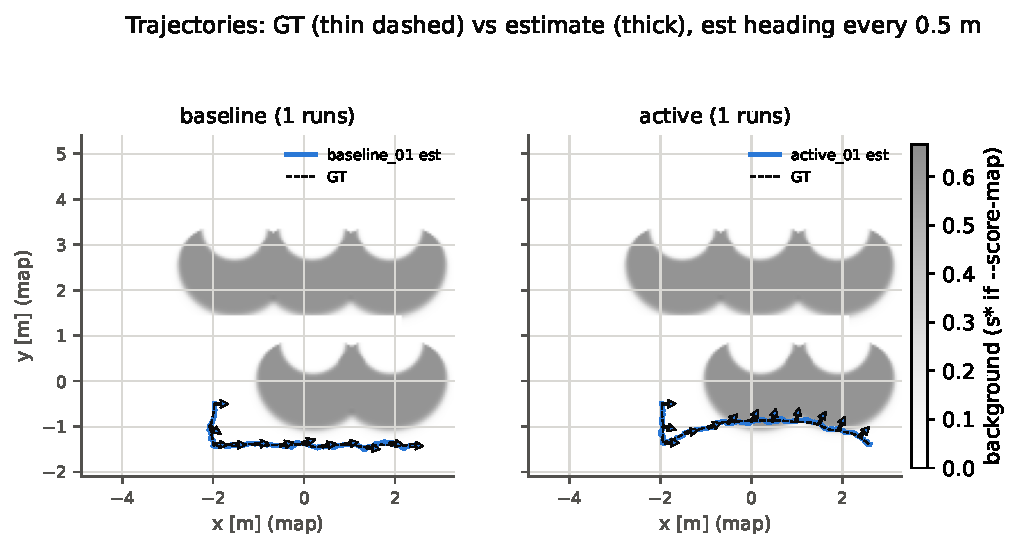
\includegraphics[height=3.2cm,trim=0 0 0 36,clip]{figures/trajectories.pdf}\hfill
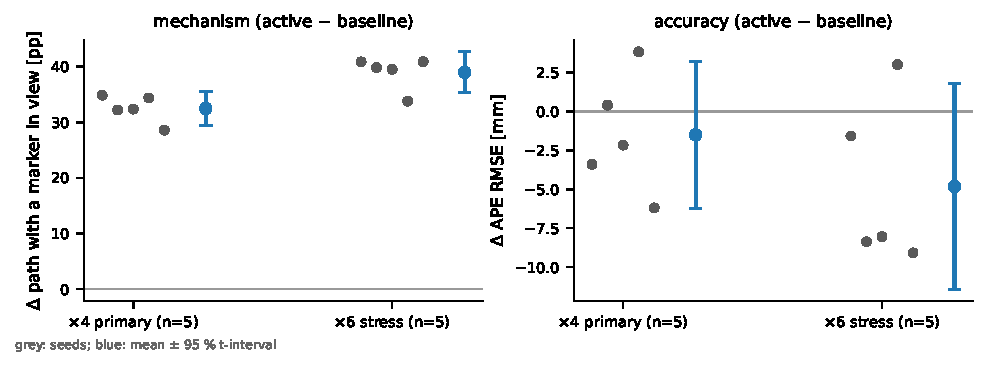
\includegraphics[height=3.2cm]{figures/paired_t010b.pdf}
\caption{(a, слева) Демонстрация рычага маршрута (один прогон): baseline идёт по $y=-1.4$\,м и не видит маркеров; active отклоняется на 0.5\,м в полосу высокого $s^*$ (серая) и смотрит на маркеры (стрелки). (b, справа) Парные разности active $-$ baseline по сидам (серые), среднее и 95\,\% $t$-интервал (синие).}
% src (a): runs/d6_20261019_055924/plots/trajectories.pdf (_team/final_inputs/trajectories.pdf; suptitle cropped); caption: _team/final_inputs/08_final_findings.md §4
% src (b): knowledge/figures/paired_t010b.pdf (scripts/t011_paired_plot.py; _team/final_inputs/paired_t010b.pdf); 08 §4, 07 §B10
\label{fig:results}
\end{figure*}

\textbf{Рычаг курса: ДП по курсу.} Путь Theta* передискретизируется с шагом 0.20\,м, и ДП Витерби по $B=36$ бинам курса $\psi_b$ выбирает курс в каждой точке ($\phi_j$~--- направление движения):
% src: _team/tasks/T-009_method_impl.md §4 (step 0.20 m, B = 36)
\begin{gather}
\mathrm{node}(j,b)=-w_s\,\frac{s(x_j,y_j,\psi_b)}{s_{\mathrm{ref}}}+w_f\,(1-\cos(\psi_b-\phi_j)),\nonumber\\
\mathrm{edge}(j,a{\to}b)=w_{sm}\Delta\psi^2+w_{lim}\max(0,|\Delta\psi|-k\,ds_j)^2,
\end{gather}
$\Delta\psi=\mathrm{wrap}(\psi_b-\psi_a)$; начальный и конечный курс закреплены штрафом $10^6(1-\cos)$; $k\approx\omega_{\max}/v_{\mathrm{cruise}}$~--- предел скорости поворота на метр (табл.~\ref{tab:params}).
% src: _team/tasks/T-009_method_impl.md §4 v2 (parameter table; k = 2.0 rad/m = wz_max 1.0 / v_cruise ~0.5 m/s [estimate, ENG measures v_cruise in T-009d])
Глобальное ДП (а не жадный выбор ActLoc) нужно из-за ограниченной скорости поворота: поворот на 90\textdegree{} занимает $\approx\pi/(2k)\approx0.8$\,м пути~--- сравнимо с окном видимости маркера ($\pm1.2$\,м), и курс должен начать меняться \emph{до} появления маркера в кадре.
% src: pi/(2*2.0) = 0.785 m; visibility window +-1.16 m at h <= 0.95 m: 02_RESEARCH_iter2_math.md "C2 update after ENG-10"; RND review 05_report_review.md #6
Член курса \emph{ситуативен}: его вес растёт с качеством доступного маркера, как $Q_f$ в RAVPP; без маркера в кадре априорный член «вперёд» $w_f$ воспроизводит базовое поведение. Табл.~\ref{tab:papers}: что мы берём из четырёх работ и что меняем.
% src: _team/knowledge/rnd/02_RESEARCH_iter2_math.md Block D ("Check of LEAD's 3-lite against RAVPP eq. 15-16"); _team/DECISIONS.md ADR-001 (yaw trigger)
\begin{table}[t]
\centering\scriptsize
\setlength{\tabcolsep}{2.5pt}
\caption{Элементы, взятые из предшествующих работ.}
\label{tab:papers}
% src: _team/tasks/T-009_method_impl.md §8; _team/knowledge/rnd/02_RESEARCH_iter2_math.md Block D; _team/knowledge/rnd/03_GATE1_RND_recommendation.md
\begin{tabularx}{\columnwidth}{@{}l>{\raggedright\arraybackslash}X>{\raggedright\arraybackslash}X@{}}
\toprule
Работа & Что взято & Что изменено (почему) \\
\midrule
FIF~\cite{fif} & информационная оценка; курс только через видимость; сигмоида видимости; насыщение «enough is enough» & аналитически, 5 маркеров, без воксельного поля; SE(2); модель оценщика + измеренный порог детекции вместо FIM пеленга \\
RAVPP~\cite{ravpp} & отталкивание маршрута $\to$ слой стоимости; член курса с весом по качеству $\to$ стоимость узла ДП & наша оценка; без APF в KB-RRT и MPC; omni-база \\
ActLoc~\cite{actloc} & выбор курса в каждой точке пути с членом гладкости & аналитическая оценка без нейросети; Витерби вместо жадного выбора; предел скорости поворота \\
LWL~\cite{lwl} & «pixels matter» $\to$ порог по проекционной площади & без обучения (нет SfM по визуальным признакам; в RTAB-Map их нет) \\
\bottomrule
\end{tabularx}
\end{table}

\begin{table}[t]
\centering\scriptsize
\setlength{\tabcolsep}{2.5pt}
\caption{Параметры (спецификация v2; в репозитории: \texttt{active\_localization.yaml}, активные параметры Nav2).}
\label{tab:params}
% src: _team/tasks/T-009_method_impl.md v2: §1 (f, s), §2 (scorer, v2: k_A 20, r_min 0.66, k_r 40), §3 (layer), §4 (DP, v2: k 2.0 [estimate])
% A_min, r_min window from FACTS.md 18.10 (ENG-10); HFOV from FACTS (camera)
% c_max 150: DECISIONS.md (DIR 18.10 15:45); all values as in nav2_params_active.yaml (loc_layer, GridBased) used in T-010b (commit 35e1ce7, _team/final_inputs/T-010b_ENG.md)
\begin{tabularx}{\columnwidth}{@{}l>{\raggedright\arraybackslash}X@{}}
\toprule
Оценка & $f=528.4$\,пкс, $s=0.08$\,м, HFOV $=1.089$\,рад, $k_{\mathrm{fov}}=40$\,рад$^{-1}$, $A_{\min}=500$\,пкс$^2$, $k_A=20$, $r_{\min}=0.66$\,м, $k_r=40$\,м$^{-1}$, $M=1$ \\
Слой & 36 курсов, $s_{\mathrm{ref}}=0.632$, $p=1$, $c_{\max}=150$ \\
ДП & шаг 0.20\,м, $B=36$, $w_s=1.0$, $w_f=0.3$, $w_{sm}=0.5$, $k=2.0$\,рад/м, $w_{lim}=100$ \\
\bottomrule
\end{tabularx}
\end{table}

% =====================================================================
\section{Интеграция в Nav2}
% =====================================================================
\looseness=-1 Оба рычага~--- нативные C++-плагины Nav2 (рис.~\ref{fig:nav2}), поэтому BT и его восстановления \emph{идентичны} базовым. \texttt{LocalizabilityLayer}~--- дополнительный слой глобальной карты стоимости (считается раз на геометрию карты). \texttt{LocalizationAwarePlanner} зарегистрирован под id базового планировщика, оборачивает Theta* и пишет курсы ДП в путь. MPPI следует им: \texttt{PathAlignCritic.use\_path\_orientations: true} (есть в MPPI Humble 1.1.20), критики езды лицом вперёд (PathAngle, PreferForward) отключены. Для пути ДП с шагом 0.20\,м \texttt{offset\_from\_furthest} критика PathAlign снижен с 20 до 4 точек ($\approx$0.8\,м): при 20 (4\,м, за горизонтом MPPI $\approx$1.1\,м) Humble пропускает критик и игнорирует курсы. Все изменения~--- в отдельном файле параметров активного режима; базовые параметры не тронуты. Python-пакет с теми же формулами~--- тестовый оракул (golden fixtures) и средство офлайн-прогноза (\S4).
% src: _team/DECISIONS.md ADR-001 (integration), _team/tasks/T-009_method_impl.md §3-§5; FACTS.md 18.10 (ros-humble-nav2-mppi-controller 1.1.20 has use_path_orientations)
% src (offset_from_furthest 20 -> 4, ~0.8 m, horizon ~1.1 m, active params only): _team/DECISIONS.md D-8; nav2_params_active.yaml:198; commit 35e1ce7
% C++ plugins in the runs: nav2_params_active.yaml GridBased.plugin = al_nav2_plugins/LocalizationAwarePlanner (T-010b at commit 35e1ce7, T-010b_ENG.md)

\begin{figure}[t]
\centering
\begin{tikzpicture}[font=\scriptsize,
  box/.style={draw,rounded corners=1pt,align=center,inner sep=2pt,minimum height=6mm},
  ours/.style={box,fill=blue!12,draw=blue!60!black},
  lab/.style={font=\tiny,inner sep=1pt},
  >={Stealth[length=1.5mm]}]
\node[box]  (bt)    at (0,0)     {BT navigator\\(без изменений)};
\node[ours] (lap)   at (2.85,0)  {\texttt{LocalizationAware-}\\\texttt{Planner}: Theta* + ДП};
\node[box]  (mppi)  at (5.9,0)   {MPPI Omni\\(следует $\psi$)};
\node[ours] (layer) at (2.85,-0.95) {глобальная costmap +\\\texttt{LocalizabilityLayer}};
\node[box]  (lm)    at (0,-0.95)  {landmarks.yaml\\(экспорт карты)};
\node[lab]  (cmd)   at (5.9,-0.95) {\texttt{cmd\_vel} $\to$ робот};
\draw[->] (bt) -- node[lab,above]{цель} (lap);
\draw[->] (lap) -- node[lab,above]{путь + $\psi_j$} (mppi);
\draw[->] (layer) -- node[lab,right]{стоимость} (lap);
\draw[->] (lm) -- node[lab,above]{$p_i$} (layer);
\draw[->] (mppi) -- (cmd);
\end{tikzpicture}
\caption{Интеграция. Синим~--- наши плагины (C++); остальное~--- стандартный Nav2 Humble с базовым BT.}
\label{fig:nav2}
\end{figure}

% =====================================================================
\section{Эксперимент}
% =====================================================================
\looseness=-2 \textbf{Режимы.} \emph{Базовый} (baseline): стандартный Nav2 (\texttt{nav2\_params\_v2.yaml}, BT v3) без изменений. \emph{Активный} (active): тот же стек и два плагина (отдельный файл параметров). \emph{Контрольный} (control): активный стек с \texttt{null}-оценкой и выключенным слоем (\texttt{loc\_layer.enabled: false}; ДП = априорный член «вперёд»); он отделяет эффект самого стека (курсы ДП, настройки PathAlign) от эффекта оценки.
% src: _team/DECISIONS.md D-2, D-8 (control inherits offset_from_furthest 4: baseline<->control = stack, control<->active = method); _team/tasks/T-009_method_impl.md §5 v2 (RND-7 item 1)
\textbf{Сценарий и протокол.} \texttt{shelves\_loop\_a}: от позы появления $(-2.0,-0.5)$ через $(2.6,-0.8)$ и $(-0.5,2.45)$ назад к старту, 16.2\,м.
% src: navigation/src/al_eval/config/scenarios/shelves_loop_a.yaml (3 goals); 16.2 m: _team/final_inputs/summary_x4.md (path length GT 16.24/16.11/16.19 m)
Каждый прогон перезапускает симулятор, локализацию и Nav2 с чистой копией базы карты, той же начальной позой и сдвигом на 0.6\,м перед первой целью (иначе RTAB-Map стартует с последней позы в базе). Сиды 42--46; на каждом сиде три режима идут подряд с циклическим сдвигом порядка (чередование); 15 прогонов на уровень шума.
% src: _team/DECISIONS.md D-2; FACTS.md 16.10 (spawn), 18.10 (DB re-initialisation); _team/final_inputs/T-010b_ENG.md "Setup" (seeds 42-46, interleaved per seed with rotated order, 15 runs per series, 30 in total)
Первая серия (T-010: 3 сида, режимы блоками) заменена: коэффициент реального времени в ней зависел от режима (baseline 0.63, control 0.74)~--- конфаундер; при чередовании он 0.75--0.78 в 26 из 30 прогонов в каждом режиме.
% src: _team/final_inputs/07_results_draft.md §A L3 "Confound (ENG-35)" (RTF baseline 0.63 +- 0.02, control 0.74 +- 0.03); T-010b_ENG.md "Setup" (RTF 0.75-0.78 for 26/30 runs in every mode)
\textbf{Шум одометрии.} Одометрия Gazebo идеальна, и дрейф добавляется: случайное блуждание с дисперсией, растущей с путём и поворотом (по умолчанию $\sigma_x\approx5$\,см на 10\,м), ошибка масштаба 1\,\% и дрейф курса 0.01\,рад/м, умноженные на $k$; сиды во всех режимах одинаковы. $k=4$ зафиксирован до первого активного прогона пре-регистрированным правилом (D-5); $k=6$~--- стресс-уровень, добавленный после T-010. Шум курса растёт с углом поворота, так что активный режим, поворачивая больше, по построению получает больше дрейфа.
% src: _team/DECISIONS.md D-3 (rotation term penalises the turning mode, to be stated), D-5 (rule; result frozen x4, 18.10 15:50); navigation/src/al_odom_noise/config/odom_noise.yaml (defaults: k_xx 2.5e-4 m^2/m, scale_x/y 0.01, yaw_drift_per_m 0.01, k_rr 5.0e-4 rad^2/rad); x6 "added after T-010": 07_results_draft.md §B2 (D-9), 08_final_findings.md C4
% NOTE: the x4/x6 multiplier is applied by ENG's run script (eng/19_overnight_t010b.sh, not in this repo); which parameters it scales is not restated here.
\textbf{Метрики.} Истина~--- поза из Gazebo, оценка~--- \texttt{map}$\to$\texttt{base\_link}. APE и RPE (трансляция, $xy$, RPE через 1\,м) в evo 1.38 \emph{без выравнивания}: выравнивание Умеямы скрывает дрейф.
% src: eval/README.md; FACTS.md 16.10 (evo 1.38, alignment hides drift: 0.173 -> 0.072 m on synthetic data)
Механизм: доля пути с маркером в кадре ($\ge1$ принятая детекция за последнюю секунду), наибольший слепой участок, детекции на метр. Вторичные: коррекции \texttt{map}$\to$\texttt{odom}, время, длина пути, поворот, достигнутые цели.
% src: 07_results_draft.md §A L1 (path share metric, 1 s window, longest blind arc), §B3 (primary/secondary outcomes); eval/README.md §7 (summary.csv columns)
Все ряды обрезаны до [старт первой цели, конец последней] (без стартовой релокализации), а коррекции \texttt{map}$\to$\texttt{odom} отсчитываются от тождественного преобразования: одометрия стартует из истинной позы.
% src: eval/README.md §7 (T-011c: cropping on, --map-odom-ref zero by default); odom_noise.yaml (init_from_gt: true); summary_x4.md header (not aligned, window result.yaml, reference identity)
\textbf{Статистика} (задана до прогонов). Единица~--- сид (одна чередующаяся тройка); приводим среднюю парную разность с 95\,\% $t$-интервалом ($n=5$) и число сидов с тем же знаком; $p$-значений нет. Основной уровень~--- ${\times}4$; ${\times}6$~--- описательный.
% src: _team/final_inputs/07_results_draft.md §B (1 unit, 2 series, 5 t-interval df 4, 7 no p-values; written before T-010b)
\textbf{Пре-регистрированный прогноз.} Python-оракул до прогонов воспроизвёл сценарий офлайн (спецификация v2, идеальное следование пути): маркер в кадре на 7\,\% пути у базового режима и $\approx$60\,\% у активного (наибольший слепой участок 8.6 против 3.7\,м). Слой не меняет маршрут loop\_a, но отклоняет прямой участок на 0.5\,м уже при $c_{\max}\approx120$; отсюда $c_{\max}=150$ и отдельная демонстрация рычага маршрута (D-6: один прогон, сид 42, ${\times}4$, прямой участок на $y=-1.4$\,м ниже рядов маркеров).
% src: _team/predict_v2/prediction.md (T-011b v2): n_eff>=0.5 frac L 0.074 (baseline) vs 0.616 (active; s>=0.5: 0.604), longest gap 8.61 vs 3.66 m; c_max sweep: loop_a dL -0.0 % up to 80, -0.8 % at 160; straight-leg probe offset 0.53 m at c_max 120
% src (demo): _team/final_inputs/T-010b_ENG.md "D-6" (runs/d6_20261019_055924, seed 42, x4, shelves_south_wall.yaml, leg 2 planned straight line y = -1.4); DECISIONS.md D-6 option (b)

% =====================================================================
\section{Результаты}
% =====================================================================
% Text: RND final, _team/final_inputs/08_final_findings.md §3 "§5 Results" (verbatim; only the Table/Fig. references are added)
\looseness=-1 Достигнуты все 90 целей основного эксперимента (loop\_a, 5 сидов $\times$ 3 режима, чередование внутри сида; шум одометрии ${\times}4$ по пре-регистрации и ${\times}6$ как добавочный стресс-уровень).
% src: T-010b_ENG.md "Setup" (90/90 goals); summary_x4.md, summary_x6.md (goals reached 15/15 per mode)
Метод меняет то, что видит робот, как и предсказано офлайн. Доля пути с маркером в кадре выросла с 33 до 66\,\% при ${\times}4$ (прогноз 60\,\%; +32\,п.\,п., 95\,\% ДИ [+29, +36], 5/5 сидов; табл.~\ref{tab:results}, рис.~\ref{fig:results}b), детекций в 4.7 раза больше, наибольший слепой участок сократился с 4.9 до 3.3\,м.
% src: 08_final_findings.md C1 (33 -> 66 %, +32 pp [+29, +36], 5/5, predicted 60 %, detections x4.7, blind arc 4.9 -> 3.3 m); 07_results_draft.md §D1; det/m 3.0 -> 14.1: summary_x4.md
Контрольный режим остался на уровне базового. Если с запланированного маршрута маркеры не видны, слой сдвигает его в полосу маркеров (рис.~\ref{fig:results}a: объезд 0.5\,м, 0\,$\to$\,69 детекций, +2\,с).
% src: 08 C1 (control ~ baseline; path share 22 %, det/m 3.3: 07 §D3, summary_x4.md); 08 C2 / T-010b_ENG.md D-6 (y -1.24 ... -0.86, bends 0.54 m; detections 0 -> 69; +0.15 m, +2.1 s)
Точность при ${\times}4$ измеримо не изменилась: APE RMSE $\Delta=-1.5$\,мм [$-6.2$, $+3.2$] (базовый 40\,мм), т.\,е.\ выигрыш не более 6\,мм.
% src: 08 C3 (-1.5 mm [-6.2, +3.2], 3/5; upper bound 6.2 mm ~ 16 %); baseline 0.040 m: summary_x4.md
При ${\times}6$ оценки эффекта растут: APE RMSE $-4.8$\,мм [$-11.4$, $+1.8$], APE max $-22$\,мм (5/5), а наибольший скачок локализации на 9\,см меньше, чем в контроле (5/5). Цена~--- +23\,\% (${\times}4$) и +30\,\% (${\times}6$) времени.
% src: 08 C4 (APE RMSE -4.8 [-11.4, +1.8], 4/5; APE max -21.6 [-38.5, -4.7], 5/5), C5 (map->odom max step active - control -0.089 m [-0.163, -0.016], 5/5), C7 (time +8.2 s +23 % at x4, +12.1 s +30 % at x6, 5/5)

% =====================================================================
\section{Обсуждение, ограничения, улучшения}
% =====================================================================
% Text: RND final, _team/final_inputs/08_final_findings.md §3 "§6 Discussion" (verbatim)
\looseness=-1 На этой карте лидарный ICP удерживает ошибку около 4\,см. Ограничения от ориентиров в основном избыточны, и ошибка не падает, пока маркер в кадре. Польза от взгляда на маркеры видна лишь с ростом дрейфа, что согласуется с ролью маркеров как резерва при запаздывании коррекций ICP.
% src: 08 C8 [hypothesis] (active x4: APE 0.043 m with a marker in view vs 0.031 m without; effect appears only with more drift); baseline APE RMSE 40 / 54 mm: summary_x4.md, summary_x6.md
Контрольный режим при ${\times}4$ был немного точнее базового ($-2.7$\,мм): часть любой разницы даёт само следование пути с учётом курса.
% src: 08 C6 (control - base APE RMSE -2.7 mm [-4.8, -0.6], 5/5)
Ограничения: один сценарий, 5 сидов, симуляция; ${\times}6$ добавлен после первой серии; демонстрация маршрута~--- один прогон; модель детекции подобрана по одному маркеру. Улучшения: член курса с включением по неопределённости ради сокращения времени, член вырожденности лидара в оценке, испытания в бедных для ICP коридорах.
% src: 08 §3; FACTS.md 18.10 (ENG-10 detection model fitted on one marker); DECISIONS.md D-7 (lidar-degraded condition deferred)

% ---------------------------------------------------------------------
% Table 3: x4 summary from eval/summarize.py (_team/final_inputs/summary_table.tex = runs/t010b_20261019_055924/x4/summary/summary_table.tex, 7 rows)
% + row "Path with marker in view" + column "Delta active - base [95 % CI]" (08 §4, 07 §D3 "Table 2").
% Changes vs the generated file: APE in mm instead of m (0.040 m = 40 mm, same digits); std columns kept.
% Inlined (not \input) because of the extra row/column; eval_out/summary_table.tex is no longer read.
\begin{table}[t]
\centering\scriptsize
\setlength{\tabcolsep}{1.1pt}
\caption{Шум ${\times}4$ (основной): среднее $\pm$ СКО, 5 сидов; $\Delta$: средняя парная разность active $-$ baseline, 95\,\% $t$-интервал. Прочее~--- в репозитории.}
\label{tab:results}
\begin{tabular}{@{}lcccc@{}}
\toprule
Метрика & baseline & active & control & $\Delta$ [95\,\% ДИ] \\
\midrule
% src: 08_final_findings.md §4 (33 / 66 / 22), C1 (+32 pp [+29, +36]); 07_results_draft.md §D1, §D3
Путь с маркером [\%] & 33 & 66 & 22 & $+32$\,[$+29$,\,$+36$] \\
% src: summary_table.tex rows (x4); Delta CIs: 07_results_draft.md §D3 "Table 2" line, 08 C3
APE RMSE [мм] & $40\!\pm\!2$ & $39\!\pm\!3$ & $37\!\pm\!1$ & $-1.5$\,[$-6.2$,\,$+3.2$] \\
APE max [мм] & $119\!\pm\!21$ & $117\!\pm\!12$ & $109\!\pm\!25$ & $-1.9$\,[$-31$,\,$+27$] \\
Детекций на м & $3.0\!\pm\!0.8$ & $14.1\!\pm\!0.7$ & $3.3\!\pm\!0.7$ & $+11.1$\,[$+9.6$,\,$+12.6$] \\
Max $|$\texttt{map}$\to$\texttt{odom}$|$ [м] & $1.279\!\pm\!0.557$ & $1.083\!\pm\!0.299$ & $1.069\!\pm\!0.335$ & $-0.20$\,[$-0.96$,\,$+0.57$] \\
% src: time CI 08 C7 / 07 §D3; path length Delta -0.132 (5/5): summary_x4.md "Paired by seed" (no CI computed by RND)
Время [с] & $36.0\!\pm\!1.9$ & $44.2\!\pm\!2.0$ & $40.5\!\pm\!0.9$ & $+8.2$\,[$+6.9$,\,$+9.4$] \\
Длина пути [м] & $16.2\!\pm\!0.0$ & $16.1\!\pm\!0.1$ & $16.2\!\pm\!0.0$ & $-0.13$ (5/5) \\
Цели достигнуты & 15/15 & 15/15 & 15/15 & -- \\
\midrule
% src: summary_x6.md (APE RMSE 0.054 / 0.049 / 0.053 m, APE max 0.160 / 0.138 / 0.159 m); 08 §4
\multicolumn{5}{@{}p{\linewidth}@{}}{${\times}6$ (стресс): APE RMSE 54 / 49 / 53\,мм, APE max 160 / 138 / 159\,мм.} \\
\bottomrule
\end{tabular}
\end{table}
\vspace{-2pt}
\scriptsize
\begin{thebibliography}{9}\setlength{\itemsep}{0pt}
\bibitem{fif} \foreignlanguage{english}{Z.~Zhang, D.~Scaramuzza, ``Fisher Information Field: an Efficient and Differentiable Map for Perception-aware Planning,'' arXiv:2008.03324, 2020.}
\bibitem{lwl} \foreignlanguage{english}{L.~Di~Giammarino et al., ``Learning Where to Look: Self-supervised Viewpoint Selection for Active Localization using Geometrical Information,'' arXiv:2407.15593, 2024.}
\bibitem{ravpp} \foreignlanguage{english}{S.~Barlakas et al., ``Robot Active Vision-Based Path Planning for Localization Improvement in Indoor Environments,'' in Proc.\ IEEE/RSJ IROS, 2024.}
\bibitem{actloc} \foreignlanguage{english}{J.~Li et al., ``ActLoc: Learning to Localize on the Move via Active Viewpoint Selection,'' in Proc.\ CoRL, 2025.}
\end{thebibliography}
% src (references): first pages of the PDFs in docs/ (arXiv ids, IROS 2024 header, CoRL 2025 footer)

\end{document}
